\documentclass[pdf,table]{beamer}
\usepackage{graphicx,hyperref,pdfpages}
\usepackage{tikz}
\usepackage{textpos}
\usepackage{longtable}
\usepackage{listings}
\usepackage{colortbl}
%\usepackage[table]{xcolor}
%\usepackage{multirow}
\usetikzlibrary{arrows}
\usetikzlibrary{positioning,chains,fit,shapes,calc}
\usetikzlibrary{mindmap}
\usepackage{tikz-uml}

%defin colours
\definecolor{codegreen}{rgb}{0,0.6,0}
\definecolor{codegray}{rgb}{0.5,0.5,0.5}
\definecolor{codepurple}{rgb}{0.58,0,0.82}
\definecolor{backcolour}{rgb}{0.95,0.95,0.92}
\definecolor{delim}{rgb}{20,105,176}



\lstdefinelanguage{CTO}{
	keywords={abstract, asset, by, concept, default, enum, event, identified, Integer, o, participant, String, transaction },
	comment=[l]{//},
	comment=[s]{/*}{*/},
	string=[b]",
	sensitive=true,
}

\lstdefinelanguage{ACL}{
	keywords={transaction,condition,rule,description,participant,operation,resource,action,ALLOW,READ,ALL,CREATE,UPDATE,DELETE,ANY,DENY},
	comment=[l]{//},
	comment=[s]{/*}{*/},
	string=[b]",
	sensitive=true,
}

%define Javascript language
\lstdefinelanguage{JavaScript}{
keywords={typeof, new, true, false, catch, function, return, null, catch, switch, var, if, in, while, do, else, case, break},
keywordstyle=\color{blue}\bfseries,
ndkeywords={class, export, boolean, throw, implements, import, this},
ndkeywordstyle=\color{darkgray}\bfseries,
identifierstyle=\color{black},
sensitive=false,
comment=[l]{//},
morecomment=[s]{/*}{*/},
commentstyle=\color{purple}\ttfamily,
stringstyle=\color{red}\ttfamily,
morestring=[b]',
morestring=[b]"
}
%define json language
\colorlet{punct}{red!60!black}
\definecolor{background}{HTML}{EEEEEE}
\definecolor{delimiter}{RGB}{20,105,176}
\colorlet{numb}{magenta!60!black}

\lstdefinelanguage{json}{
    numbers=left,
    numberstyle=\scriptsize,
    stepnumber=1,
    numbersep=8pt,
    showstringspaces=false,
    breaklines=true,
    frame=lines,
    backgroundcolor=\color{background},
    literate=
     *{0}{{{\color{numb}0}}}{1}
      {1}{{{\color{numb}1}}}{1}
      {2}{{{\color{numb}2}}}{1}
      {3}{{{\color{numb}3}}}{1}
      {4}{{{\color{numb}4}}}{1}
      {5}{{{\color{numb}5}}}{1}
      {6}{{{\color{numb}6}}}{1}
      {7}{{{\color{numb}7}}}{1}
      {8}{{{\color{numb}8}}}{1}
      {9}{{{\color{numb}9}}}{1}
      {:}{{{\color{punct}{:}}}}{1}
      {,}{{{\color{punct}{,}}}}{1}
      {\{}{{{\color{delimiter}{\{}}}}{1}
      {\}}{{{\color{delimiter}{\}}}}}{1}
      {[}{{{\color{delimiter}{[}}}}{1}
      {]}{{{\color{delimiter}{]}}}}{1},
}
%\lstdefinelanguage{json}{
%    numbers=left,
%    numberstyle=\scriptsize,
%    stepnumber=1,
%    numbersep=8pt,
%    showstringspaces=false,
%    breaklines=true,
%    frame=lines,
%    backgroundcolor=\color{backcolour},
%    literate=
%     *{\{}{{{\color{delim}{\{}}}}{1}
%      {\}}{{{\color{delim}{\}}}}}{1}
%      {[}{{{\color{delim}{[}}}}{1}
%      {]}{{{\color{delim}{]}}}}{1},
%}



\lstdefinestyle{mys}{
	backgroundcolor=\color{backcolour},
	commentstyle=\color{codegreen},
	keywordstyle=\color{magenta},
	stringstyle=\color{codepurple},
	numberstyle=\color{codegray},
	basicstyle=\ttfamily\tiny,
	breakatwhitespace=false,
	breaklines=true
	captionpos=b,
	keepspaces=true,
	numbers=left,
	numbersep=5pt,
	showspaces=false,
	showstringspaces=false,
	showtabs=false,
	tabsize=2}
\lstset{style=mys}



\tikzset{every matrix/.style={ampersand replacement=\&,column sep=1.75cm,row sep=2cm},
		BTWMat/.style={ampersand replacement=\&, column sep=0.75cm,row sep=1cm},
		eulerMat/.style={ampersand replacement=\&,column sep=1.1cm,row sep=2cm},
		vertexHighlight/.style={circle,fill=red!80,inner sep=.1cm,text=white},
		vertex/.style={circle,fill=blue!80,inner sep=.1cm,text=white},
		bank/.style={rectangle,fill=blue!50,inner sep=0.1cm,text=black!80}
		edge/.style={--,line width=2pt},
		Dedge/.style={->,line width=2pt},
		DedgeT/.style={->,line width=1pt},
		BiEdge/.style={<->,line width=2pt},
		BiEdgeT/.style={BiEdge,line width=1pt},
		edgeHighlight/.style={--,line width=2pt,color=red},
		loop/.style={min distance=10mm, line width=2pt},
		loopT/.style={min distance=-10mm, line width=1pt},
		label/.style = { rectangle, rounded corners, draw,
		                 minimum width = 2em, fill = yellow!50,
		                 text = red, font = \tiny\bfseries },
		labelT/.style = { circle, draw, line width=1pt,
		                 minimum width = 1em, fill = yellow!50,
		                 text = red, font = \tiny\bfseries },
		every node/.style={align=center}}



\newcommand{\cwideadline}{3$^{rd}$ November 2019}
\newcommand{\cwiideadline}{5$^{th}$ January 2020}
%\newcommand{\cwiiideadline}{31$^{st}$ March 2017}
%\newcommand{\cwiiideadline}{15$^{th}$ April 2018}
\newcommand{\resitdeadline}{1$^{st}$ August 2020}
\newcommand{\deferraldeadline}{1$^{st}$ August 2020}
\newcommand{\deferraldeadlineMay}{1$^{st}$ May 2020}
\newcommand{\moduleCode}{CST4025}
\newcommand{\moduleLeader}{Dr Ian Mitchell }
\newcommand{\theauthor}{Dr Ian Mitchell }
\newcommand{\academicyear}{2019-20}
\newcommand{\email}{i.mitchell@mdx.ac.uk}
\newcommand{\moduleTitle}{Blockchain Development}
\newcommand{\office}{T108}
\newcommand{\officehours}{Autumn \& Winter Terms: Tuesdays 1515-1615hrs; and, Wednesdays 1415-1515hrs}
\newcommand{\tel}{0208-411-6014}
\newcommand{\deptName}{Computer Science}
%\newcommand{\officehours}{Friday 1100\--1300hrs Autumn Term \\ Thursday 1400\--1600hrs Winter Term}
%\newcommand{\officehours}{Autumn Term: Mondays 1300\--1500hrs \\ Winter Term: Thursdays 1400\--1600hrs

\def\bitcoinA{%
  \leavevmode
  \vtop{\offinterlineskip %\bfseries
    \setbox0=\hbox{B}%
    \setbox2=\hbox to\wd0{\hfil\hskip-.03em
    \vrule height .3ex width .15ex\hskip .08em
    \vrule height .3ex width .15ex\hfil}
    \vbox{\copy2\box0}\box2}}




\usepackage[style=numeric,backend=biber]{biblatex}
\addbibresource{../CST4025.bib}
\setbeamertemplate{bibliography item}{\insertbiblabel}



\mode<presentation>{
\usetheme{Madrid}
\usecolortheme{beaver}
}


\newcommand{\theweek}{9}
\renewcommand{\theequation}{\theweek.\arabic{equation}}

\title[\moduleCode:L\theweek]{\moduleTitle \\ Week: \theweek \\ Title: Smart Contracts} 

%[\includegraphics[scale=0.2]{../logo/mdxSmall}]
\institute[]{\includegraphics[scale=0.25]{../../../logo/mdxSmall} \\ Middlesex University, \\Dept. of Computer Science, \\London}
\author[\email]{\moduleLeader}
\date{\today}




\begin{document}
	\begin{frame}
		\titlepage
	\end{frame}


\addtobeamertemplate{frametitle}{}{%
\begin{textblock*}{100mm}(.94\textwidth,-0.85cm)
\includegraphics[scale=0.1]{../../../logo/transparent}
\end{textblock*}}

\begin{frame}{Lecture Objectives}
	\begin{itemize}
		\item Blockchain
		\item permissionless
		\item permission
		\item Smart contracts
	\end{itemize}	
\end{frame}

\begin{frame}{Smart Contracts }
	\begin{columns}[T]
		\begin{column}{0.60\textwidth}
			\begin{block}<1->{Definition 1 \cite{bashir2018}
}
					business rules and a state 			\end{block}
			\begin{block}<3->{Definition 2 \cite{szabo1997formalizing}}
					A smart contract is a secure and unstoppable computer program representing a n agreement that is automatically executable and enforceable 
			\end{block}
			
			\begin{block}<5->{Definition 3 }
					Business Logic \& State: Smart contracts are executed when pre-conditions are met and can allow automatic ledger updates.
			\end{block}
		\end{column}
		\begin{column}{0.40\textwidth} {\bf Key points}
			\begin{itemize}
				\item<2-> State change
				\item<3-> Enforceable
				\item<4-> Unstoppable
				\item<4-> Automatic
				\item<5-> Pre-conditions
				\item<6-> Updates
				\item<6-> Disintermediation
				\item<6-> Code is Law (Semantically sound)
				\item<6-> Fault tolerant
				\item<6-> Secure
				\item<6-> Intervention?  % e.g. medical
			\end{itemize}
		\end{column}
	\end{columns}	
\end{frame}

\begin{frame}{Smart Contracts}{Principles}
	\begin{columns}[T]
		\begin{column}{0.48\textwidth}
			\begin{itemize}
				\item Code is not understood %by everyone
				\item Code understood by humans \& machine
				\item Combination of SC and NL %Smart Contracts (SC); Natural Language (NL)
				\item Mark-up languages
					\begin{itemize}
						\item Legal Knowledge Interchange Format
						\item XML Schema
					\end{itemize}
				\item SC's are inherently deterministic
				\item Any Node must get same result
			\end{itemize}
		\end{column}
		\begin{column}{0.48\textwidth}
			\begin{itemize}
			\item Issues:
					\begin{itemize}
						\item floating points can be calculated differently in OS or Browsers
						\item JS math functions can be calculated differently
					\end{itemize}
				\item If the result is different then discordance
				\item No consensus and BC fails %Blockchain
				\item Non-deterministic functions are not permitted
				\item Programs need to be reliable and stable
			\end{itemize}
		\end{column}
	\end{columns}	
\end{frame}

\begin{frame}{Smart}
	\begin{block}<1|only@1>{Definition {\it adj.} \cite{collinsDictionary}}
		\begin{enumerate}
			\item astute, as in business; clever or bright
			\item quick, witty, and often impertinent in speech
			\item well-kept, neat
		\end{enumerate}
		\vdots
	\end{block}
	\begin{block}<2->{Misnomer}
		\begin{itemize}
			\item Deterministic
			\item Does not think
			\item it is not astute
			\item Smart?
				\begin{itemize}
					\item<3-> Disintermediation
					\item<3-> Arbitration
					\item<3-> Automation
					\item<3-> Third parties
					\item<3-> Unstoppable
					\item<3-> Enforceable
					\item<3-> Secure
					\item<3-> Compliant
					\item<3-> Legal?
				\end{itemize}
		\end{itemize}
	\end{block}
\end{frame}

\begin{frame}{Ricardian Contract \cite{grigg2004ricardian}}
	\begin{columns}[T] % 
		\begin{column}{0.48\textwidth}
			\begin{itemize}
				\item Understood by Computer and Law
				\item Address challenge of issuance of value over internet
				\begin{itemize}
					\item A contract offered by issuer to holder
					\item A valuable right held by holders and managed by the issuer
					\item Concise and readable 
					\item Signed
					\item Keys 
					\item Unique
					\item Secure
				\end{itemize}
			\end{itemize}
		\end{column}
		\begin{column}{0.48\textwidth}
			{\bf Bowtie Model\cite{bashir2018}}
			\begin{tikzpicture}[scale=1.0]
				\umlclass[x=0,y=8,name=wol]{World of Law}
				{
					\rule{20mm}{1mm}\\ 
					\rule{20mm}{1mm}\\ 
					\rule{20mm}{1mm}\\ 
					\rule{20mm}{1mm}\\ 
					\rule{20mm}{1mm}\\ 
					\rule{20mm}{1mm}\\ 
					\rule{20mm}{1mm}\\ 
					\rule{20mm}{1mm}\\ 
					\rule{20mm}{1mm}\\ 
					\rule{20mm}{1mm}\\ 
			
				}{PGP Signature}	
			\end{tikzpicture}
		\end{column}
	\end{columns}	
\end{frame}

\begin{frame}{Bowtie Model (adpated from \cite{bashir2018,grigg2004ricardian})}
	\begin{tikzpicture}[scale=1.0]
		\umlclass[x=0,y=8,name=wol]{World of Law}
		{
			\rule{20mm}{1mm}\\ \rule{20mm}{1mm}\\ 
			\rule{20mm}{1mm}\\ 
			\rule{20mm}{1mm}\\ 
			\rule{20mm}{1mm}\\ 
			\rule{20mm}{1mm}\\ 
			\rule{20mm}{1mm}\\ 
			\rule{20mm}{1mm}\\ 
			\rule{20mm}{1mm}\\ 
			\rule{20mm}{1mm}\\ 
	
		}{PGP Signature}	
		\umlclass[x=4,y=8,name=hash]{Hash}{0ea4856d3d9b97\ldots}{}
		\umlassoc[anchor1=north east,anchor2=north west,name=assoc1]{World of Law}{Hash}
		\umlassoc[anchor1=south east,anchor2=south west,name=assoc2]{World of Law}{Hash}
		\node[vertex] at (7,8) (1){};
		\node[vertex] at (7.75,8.5) (2){};
		\node[vertex] at (7.75,7.5) (3){};
		\node[vertex] at (8.50,8.50) (4){};
		\node[vertex] at (8.50,7.70) (5){};
		\node[vertex] at (8.50,9.20) (6){};
		\node[vertex] at (8.50,6.80) (7){};

		\node[vertex] at (9.250,9.25) (10){};
		\node[vertex] at (9.250,9.95) (11){};
		\node[vertex] at (9.250,8.75) (12){};
		\node[vertex] at (9.250,8.30) (13){};

		\node[vertex] at (9.250,7.40) (14){};
		\node[vertex] at (9.250,7.80) (15){};
		\node[vertex] at (9.250,6.00) (16){};
		\node[vertex] at (9.250,6.80) (17){};
		
		\draw (1) -- (2);
		\draw (1) -- (3);
		\draw (2) -- (4);
		\draw (2) -- (6);
		\draw (3) -- (5);
		\draw (3) -- (7);

		\draw (4) -- (12);
		\draw (4) -- (13);
		\draw (6) -- (10);
		\draw (6) -- (11);

		\draw (5) -- (14);
		\draw (5) -- (15);
		\draw (7) -- (16);
		\draw (7) -- (17);
		
		\draw (Hash) -- (1);

	\end{tikzpicture}
\end{frame}

\begin{frame}{Smart Contracts?}%p268-269 Bashir
	\begin{columns}[T]
		\begin{column}{0.48\textwidth}
			\begin{itemize}
				\item Law
				\item Accountancy
				\item Genesis
				\item Each TX includes Hash
				\item Is Ricardian Smart?
				\item<2-> Ricardian are different
					\begin{itemize}
						\item<2-> Enforceable
						\item<2-> Unstoppable
						\item<2-> Automatic
						\item<2-> pre-conditions
					\end{itemize}
				\item<2-> Semantic richness
				\item<2-> Contract is attached
			\end{itemize}
		\end{column}
		\begin{column}{0.48\textwidth}
			{\bf Smart Contracts}
			\begin{itemize}
				\item<3-> Denotational Semantics %indicate or designate a meaning; act of denoting; indication
					\begin{itemize}
						\item<4-> real-world
						\item<4-> meaning of the full contract
					\end{itemize}
				\item<4-> Operational Semantics %
					\begin{itemize}
						\item<5-> Execution
						\item<5-> Correctness
						\item<5-> Safety
					\end{itemize}
				\item<6-> Smart Legal Contract % have both
				\item<7-> Difference
					\begin{itemize}
						\item \bitcoinA, operational
						\item Ricardian, denotional
					\end{itemize}
			\end{itemize}	
		\end{column}
	\end{columns}	
\end{frame}

\begin{frame}{Smart Legal Contracts (adapted from \cite{grigg2015ricardian})}
	\centering
	\begin{tikzpicture}
		\node [zero] at (0,-0.250) (0x){};
		\node [zero] at (0,5) (y){};
		\node [zero] at (5,0) (x){};
		\node [zero] at (-0.250,0) (0y){};
		\draw[line width=5pt,Dedge]	(0x) -- (y);
		\draw[line width=5pt,Dedge]	(0y) -- (x);
		\node[rotate=90] at (-0.5,2) (yAxisLabel){Ricardian};
		\node at (2,-0.5) (xAxisLabel){Smart};
		\node<2-> at (1.25,4) (increaseRicardian){Increase\\Semantic\\Richness};
		\node<2-> at (4,0.75) (increasePerformance){Increase\\Automonous};
	\end{tikzpicture}
\end{frame}

\begin{frame}{Smart Contract Templates \cite{clack2016smart,clack2016asmart} }
	\begin{columns}[T]
		\begin{column}{0.48\textwidth}
			\begin{itemize}
				\item Prose
				\item Parameter
				\item Code
				\item Common Language for Augmented Contract Knowledge (CLACK)
				\item Domain Specific Language (DSL)
				\item General-purpose Programming Languages (GPL)
				
			\end{itemize}
		\end{column}
		\begin{column}{0.48\textwidth}
			\begin{itemize}
				\item DSL needed to write Smart Contracts
				\item Ethereum
					\begin{itemize}
						\item Solidity
						\item Vyper
					\end{itemize}
				\item Non-programmers
				\item graphical DSL
				\item convert semantics to code
				\item Flow, process
				\item deployed to BC
				\item Tibco StreamBase (Java-based)
			\end{itemize}
		\end{column}
	\end{columns}	
\end{frame}


\begin{frame}{Oracles} %p272 bashir
	\begin{columns}[T]
		\begin{column}{0.48\textwidth}
			\begin{itemize}
				\item SC Limitations
				\item Access to external data
				\item Provide data to SC
				
			\end{itemize}
			\begin{block}<2->{Oracle Definition }
				An Oracle is an interface that delivers data from an external source to smart contracts \cite{bashir2018}
			\end{block}
		\end{column}
		\begin{column}{0.48\textwidth}
			{\bf Examples}
			\begin{itemize}
				\item<3-> Weather reports
				\item<3-> Stock exchange
				\item<3-> IoT
				\item<4-> {\bf Changes}
				\item<4-> Authentic
				\item<4-> Trusted
				\item<4-> SC registers with Oracle
				\item<4-> Integrity
				\item<4-> Back to Centralisation?
				\item<5-> Decentralise Oracles
					\begin{itemize}
						\item source data derived from multiple sources
						\item consensus applied 
						\item authenticity
					\end{itemize}
				\item<6-> \url{provable.xyz}
			\end{itemize}
		\end{column}
	\end{columns}	
\end{frame}

\begin{frame}{Oracles (adapted from \cite{bashir2018})}
	\centering
	\begin{tikzpicture}
		\node at (0,7) (1) {Data 1};
		\node at (0,4) (2) {Data 2};
		\node at (0,1) (3) {Data 3};

		\node[vertex] at (2,7)(11) {1};
		\node[vertex] at (2,4)(12) {2};
		\node[vertex] at (2,1)(13) {3};

		\draw[Dedge] (1) -- (11);
		\draw[Dedge] (2) -- (12);
		\draw[Dedge] (3) -- (13);

		\node[draw,rectangle,font=\bfseries\large,minimum height=18ex,text width=8em] at (6,4) (21) { ORACLE  };

		\draw[Dedge] (11) -- (21.north west);
		\draw[Dedge] (12) -- (21.west);
		\draw[Dedge] (13) -- (21.south west);

		\node[font=\bfseries\normalsize,minimum height=20ex,text width=1em,rotate=90] at (11,3.00) (31) { BLOCKCHAIN };
		\node[zero] at (10.5,4) (41){};
		\draw (21.east) edge[Dedge, line width=4pt] node[above]{Secure\\Channel} (41);
	\end{tikzpicture}
\end{frame}


\begin{frame}{Decentralised Autonomous Organisations (DAO)}
	\begin{columns}[T]
		\begin{column}{0.48\textwidth}
			\begin{itemize}
				\item Smart Contract does not require BC
				\item Smart Contract can run on BC
				\item Why?
				\item Ethereum
				\item Hyperledger Fabric
				\item Broader applications
			\end{itemize}
		\end{column}
		\begin{column}{0.48\textwidth}
			\begin{itemize}
				\item Trust?
				\item Code is Law?
				\item Fully Autonomous
				\item Interaction
				\item Testing?
				\item Validation \& Verification of code
			\end{itemize}
		\end{column}
	\end{columns}	
\end{frame}



\begin{frame}{Use Case}%gambling would be a good practical example
	\begin{tikzpicture}[scale=1.0]
		\umlactor[x=0,y=6,scale=0.5,name=CUSTOMER]{CUSTOMER}
		\umlactor[x=10,y=2,scale=0.5,name=RESTAURANT]{RESTAURANT}
		\umlactor[x=0,y=2,scale=0.5,name=ESCROW]{ESCROW}
		\begin{umlsystem}[x=3,fill=blue!10]{Pizza}
			\umlusecase[x=2.5,y=4,name=order]{Order}
			\umlusecase[x=3,y=1,name=funds]{Funds}
			\umlusecase[x=3,y=5.5,name=preparation]{Preparation}
			\umlusecase[x=3,y=2.5,name=deliver]{Deliver}
		\end{umlsystem}
		\umlassoc{CUSTOMER}{order}
		\umlassoc{CUSTOMER}{funds}
		\umlassoc{CUSTOMER}{deliver}
		\umlassoc{ESCROW}{funds}
		\umlassoc{RESTAURANT}{preparation}
		\umlassoc{RESTAURANT}{funds}
%		\umlassoc{order}{preparation}
		%\umlinclude{preparation}{deliver}
		\draw[tikzuml dependency style] (order) to[bend left=35] (preparation);
		\draw[tikzuml dependency style] (preparation) to[bend left=35] (deliver);
		\draw[tikzuml dependency style] (deliver) to (funds);
	\end{tikzpicture}
\end{frame}


\begin{frame}{Use Case - Notes}
	\begin{itemize}
		\item order-delivery latency
		\item customer-restaurant agreement
			\begin{itemize}
				\item Order concurs
				\item Time between order and delivery
			\end{itemize}
		\item Money is transferred to intermediary
		\item Full funds are released to restaurant
			\begin{itemize}
				\item Order concurs
				\item deliver within agree time
				\item Time is decided on order, can vary 30min., 60min., etc)
			\end{itemize}
		\item Full funds are placed in escrow by customer
			\begin{itemize}
				\item on pre-conditions reached full funds released
				\item on pre-conditions breached partial funds are released to restaurant and customer
			\end{itemize}
		\item Smart Contract
	\end{itemize}
\end{frame}

\begin{frame}{Pizza}{State Transition Diagram}
	\begin{tikzpicture}[scale=1.0]
		\umlstateinitial[name=initial,x=0,y=0]
		\begin{umlstate}[name=order,x=3,y=2]
			{Order}
		\end{umlstate}
		\begin{umlstate}[name=preparation,x=7,y=2]
			{Preparation}
		\end{umlstate}
		\begin{umlstate}[name=dispatch,x=3,y=-2]
			{Dispatch}
		\end{umlstate}
		\begin{umlstate}[name=deliver,x=7,y=-2]
			{Deliver}
		\end{umlstate}
		\umlstatefinal[name=consume,x=11,y=0]
		\umltrans{initial}{order}
		\umltrans{order}{preparation}
		\umlVHVtrans{preparation}{dispatch}
		\umltrans{dispatch}{deliver}
		\umltrans{deliver}{consume}
	\end{tikzpicture}
\end{frame}

\begin{frame}{State/Event}{Order/placeOrder}
	\begin{itemize}
		\item verify order
		\item agreement:
			\begin{itemize}
				\item amount 
				\item max preparation time
				\item max delivery time
				\item remuneration for failure to prepare within the max. preparation time
				\item remuneration for failure to delivery within the max. delivery time
			\end{itemize}
		\item transfer funds to escrow
		\item create block with this information 
		\item block's state changes
	\end{itemize}
\end{frame}

\begin{frame}{State/Event}{Preparation}
	\begin{itemize}
		\item ingredients
		\item cook
		\item package
		\item update status
		\item dispatch
			\begin{itemize}
				\item prepared within agreed time
				\item claim proportion of funds
				\item prepared exceeding agreed time
				\item remuneration for failure to prepare, funds transferred
			\end{itemize}
		\item Events
		\item blockchain is updated
	\end{itemize}
\end{frame}

\begin{frame}{Pizza}{State Transition Diagram}
	\centering
	\begin{tikzpicture}[scale=1.0,font=\tiny]
		\umlstateinitial[name=initial,x=6.5,y=4,scale=0.5]
		\begin{umlstate}[entry=check,do=createSC,exit=placed,name=order,x=3,y=2]{Order}

		\end{umlstate}
		\begin{umlstate}[entry=timestamp,do=prepareOrder,exit=prepared,name=preparation,x=10,y=2]
			{Preparation}
		\end{umlstate}
		\begin{umlstate}[entry=timestamp,do=dispatchOrder,exit=dispatched,name=dispatch,x=3,y=-2]
			{Dispatch}
		\end{umlstate}
		\begin{umlstate}[name=deliver,x=10,y=-2,entry=timestamp,do=deliverOrder,exit=delivered]
			{Deliver}
		\end{umlstate}
		\umlstatefinal[name=consume,x=6.5,y=-3,scale=0.5]
		\umlHVtrans[font=\tiny,arg=placeOrder,pos=0.5]{initial}{order}
		\umltrans[font=\tiny,arg=prepareOrder,pos=0.5]{order}{preparation}
		\umlVHVtrans[font=\tiny,arg=dispatchOrder,pos=1.5]{preparation}{dispatch}
		\umltrans[font=\tiny,arg=deliverOrder,pos=0.5]{dispatch}{deliver}
		\umlVHtrans{deliver}{consume}
	\end{tikzpicture}
\end{frame}


%\begin{frame}{Enumerator Types}
%	\begin{columns}[T]
%		\begin{column}{0.48\textwidth}
%			\begin{lstlisting}
%			\end{lstlisting}
%		\end{column}
%		\begin{column}{0.48\textwidth}
%			{\bf XXX}
%		\end{column}
%	\end{columns}	
%\end{frame}
%
%

%\begin{frame}{X}
%	\begin{columns}[T]
%		\begin{column}{0.48\textwidth}
%			\begin{itemize}
%				\item XXX 
%			\end{itemize}
%		\end{column}
%		\begin{column}{0.48\textwidth}
%			{\bf XXX}
%		\end{column}
%	\end{columns}	
%\end{frame}


%\begin{frame}{}
%	\begin{columns}[T]
%		\begin{column}{0.48\textwidth}
%			\begin{lstlisting}
%			\end{lstlisting}
%		\end{column}
%		\begin{column}{0.48\textwidth}
%			{\bf XXX}
%		\end{column}
%	\end{columns}	
%\end{frame}
%
%

%\begin{frame}{X}
%	\begin{columns}[T]
%		\begin{column}{0.48\textwidth}
%			\begin{itemize}
%				\item XXX 
%			\end{itemize}
%		\end{column}
%		\begin{column}{0.48\textwidth}
%			{\bf XXX}
%		\end{column}
%	\end{columns}	
%\end{frame}

%\begin{frame}{}
%	\begin{itemize}
%		\item
%	\end{itemize}
%\end{frame}


%\begin{frame}{oracles}
%\centering
%\begin{tikzpicture}
%\end{tikzpicture}
%\end{frame}

\begin{frame}{Summary}
	\begin{itemize}
		\item Smart Contracts
		\item Ricardian Contracts
		\item Oracles
		\item DAO
		\item Verification and Validation of Smart Contracts
	\end{itemize}
\end{frame}

					
\begin{frame}[allowframebreaks]{References}
	\printbibliography
\end{frame}
	
\end{document}
